%% paper.tex


%\documentclass[pldi]{sigplanconf-pldi16}
\documentclass[10pt]{sigplanconf}
% standard LaTeX packages

% standard LaTeX packages
%\usepackage{changebar}

\usepackage{balance}
\usepackage{alltt}
\usepackage{amsmath}
\usepackage{balance}
\usepackage{booktabs}
\usepackage{fixltx2e}
\usepackage{graphicx}
\usepackage{boxedminipage}
\usepackage{hyperref}
\usepackage{nicefrac}
\usepackage{subfig}
\usepackage{xcolor}
\usepackage{setspace}
\usepackage{xspace}
\usepackage{multirow}
\usepackage{colortbl}
\usepackage{amsfonts} 
\usepackage{blindtext}
\usepackage{chngpage}
\usepackage{listings}
\usepackage{mathtools}
\usepackage{amssymb}
\usepackage{pifont}
%\usepackage{pgfplotstable}

\usepackage[linesnumbered, vlined, ruled]{algorithm2e}
% font selection
%\usepackage{courier}
%\usepackage[scaled]{helvet}
\usepackage{mathptmx}
\usepackage{times}

% custom packages for this paper
\usepackage{double-blind}
\usepackage{shared-affiliation}

\usepackage[numbers,sort&compress,square]{natbib}
\newcommand{\wenfei}[1]{\textcolor{red}{$<<$Wenfei: #1$>>$}}

\lstset{
  basicstyle=\tiny,
  columns=fullflexible,
  numbersep=5pt,
  numberstyle=\scriptsize,
  showstringspaces=false,
  escapeinside={/*@}{@*/},
  belowcaptionskip=1\baselineskip,
  language=C,
  showstringspaces=true,
  keywordstyle=\bfseries,
  commentstyle=\itshape,
}


%\pgfplotstableset{
%    color cells/.style={
%        col sep=comma,
%        string type,
%        postproc cell content/.code={%
%                \pgfkeysalso{@cell content=\rule{0cm}{2.4ex}\cellcolor{black!##10}\pgfmathtruncatemacro\number{##1}\ifnum\number>5\color{white}\fi##1}%
%                },
%        columns/x/.style={
%            column name={},
%            postproc cell content/.code={}
%        }
%    }
%}


\makeatletter
\def\@copyrightspace{\relax}
\makeatother

\captionsetup{format=default, font=bf}


\newcommand*{\Scale}[2][4]{\scalebox{#1}{$#2$}}%
\newcommand{\comment}[1]{{}}

%% taken from unknown.sty
%\DeclareCaptionType{copyrightbox}

\sloppy

\begin{document}

\title{
  Learning from Big Security
}

\input macros.tex

%\numberofauthors{2}
\authorinfo{Linhai Song}
           {University of Wisconsin--Madison}
           {\{songlh\}@cs.wisc.edu}
\maketitle
\begin{abstract}
\input section/abstract.tex
\end{abstract}


\section{Introduction}

As a free online service, VirusTotal~\cite{virustotal} analyzes files submitted by real-world users to identify many different kinds of malwares, 
like viruses, worms, trojans, and so on. 
VirusTotal applies different antivirus engines to each submitted file and generate an aggregated reports. 
All submitted files and generated reports are saved and can be accessed through public API. 

The repository on VirusTotal provides a good source to conduct data mining. 
Firstly, there are huge amount of data on VirusTotal.
Figure~\ref{fig:subnum} shows that there were more than 40 million suspicious files 
submitted last November. 
This amount of data makes VirusTotal a rough estimation of malwares in the real world. 
Secondly, all data on VirusTotal are labeled by state-of-the-art antivirus techniques. 
VirusTotal updates each antivirus engine every 5 minutes. 
Besides whether a given a submitted file is detected by an antivirus engine, VirusTotal also keeps exact detection tag returned by each engine. 
There are also online active malware researchers, 
who can comment and vote each submitted file and serve as an important supplement of antivirus engines. 
We believe mining data on VirusTotal could enable many ``Big Security'' applications. 

In industry, antivirus vendors widely use VirusTotal to identify false negatives and false positives of their products. 
They only utilize VirusTotal reports separately for each single suspicious file, but fail to leverage the whole repository. 
In academia, researchers began to pay attention to correlations among different VirusTotal reports. 
For example, {\bf [ToDo: discuss Heqing's work]}
We believe there are much more research opportunities through mining VirusTotal. 

In this paper, we view data on VirusTotal as a stream, based on each file’s submission time, and design two stream mining applications: 
\textit{hot malware family mining} and \textit{malware prediction}. 
There are possibly infinite malware families. 
Hot malware family mining can precisely identify malware families, 
which occupy more than a given percentage of total malwares, by using a constant number of counters.
Malwares does not appear uniformly across different malware families or across time, 
and they appear in bursts. 
We built a cache-based algorithm to predict malwares in which families would appear in the near future. 

\begin{figure}[t!]
\begin{center}
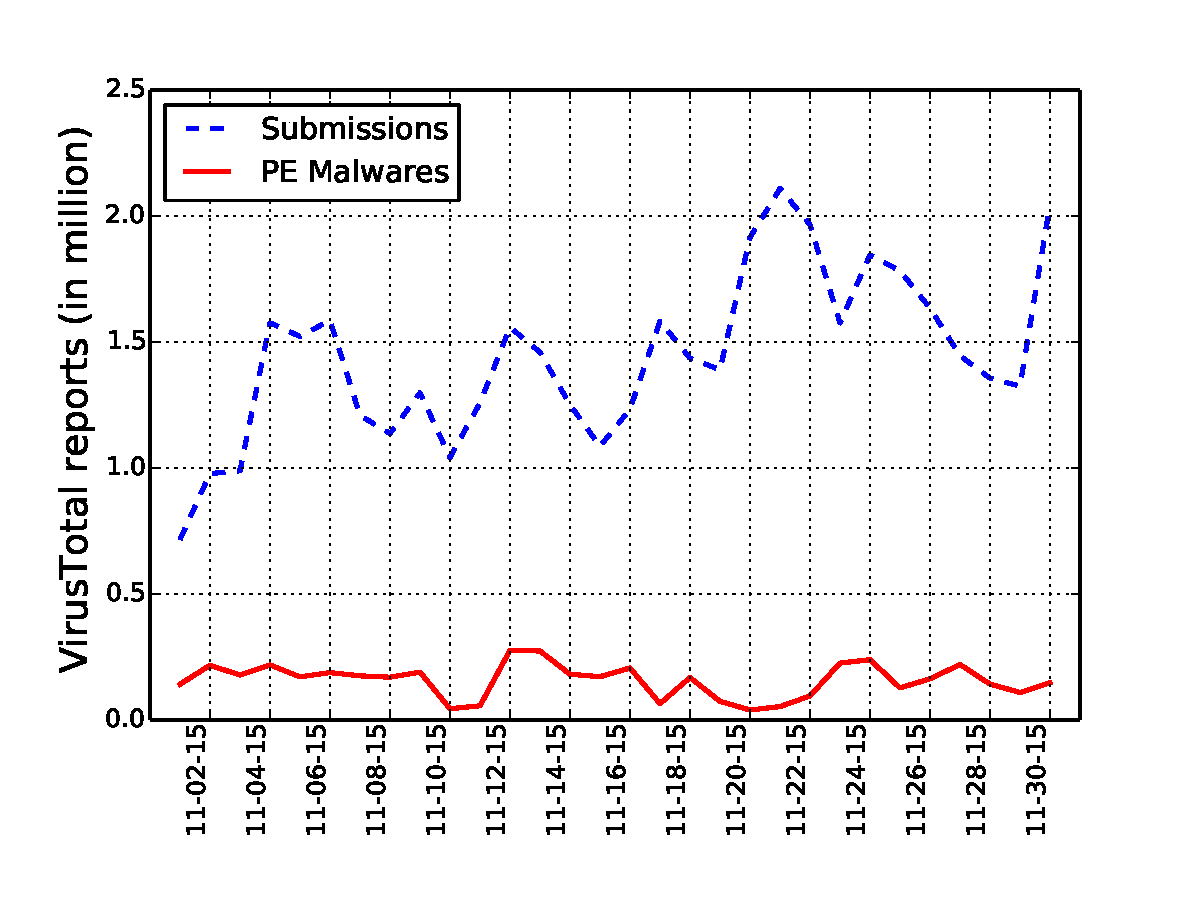
\includegraphics[width=3.0in]{figure/nov}
\caption{The number of files submitted to VirusTotal last November. }
\label{fig:subnum}
\end{center}
\end{figure}

In summary, we made the following contributions in this paper:

\begin{itemize}

\item We collect data submitted to VirusTotal last November, 
and briefly analyze these data to understand the characteristics of VirusTotal repository (Section~\ref{sec:meth}). 
\item We build two stream mining applications, one could identify hot malware family in a constant number of counters (Section~\ref{sec:hot}), 
and the other could predict malwares in the near future (Section~\ref{sec:predict}). 
Experimental results show that we can cover all hot malware family with a very few false positives, and we can predict future malwares with a high precision.
\item We discuss the future research opportunities through mining data on VirusTotal (Section~\ref{sec:oppo}), 
and demonstrate the feasibility by using our experience of building stream mining applications. 

\end{itemize}





\section{Data Collection and Basic Properties}
\label{sec:meth}

This section discusses how we collected and preprocessed data from VirusTotal.
We will present the analysis of these data in the next two sections.

\begin{table}[h!]
\centering
\footnotesize
{
%\begin{tabular}{@{\hspace{3pt}}l@{\hspace{3pt}}|@{\hspace{3pt}}c@{\hspace{3pt}}}
\begin{tabular}{l|l}
\hline
Metadata Fields & Explanation \\
\hline                            
%\cline{1-1}
{\bf name}      & file name of the submitted sample \\
{\bf timestamp} & timestamp for when the submission was made \\
{\bf source\_country} & the country from which the submission was made \\
{\bf source\_id} & user id of whom made the submission\\
{\bf tags} & providing more specific information for each {\bf type}\\
{\bf link} & where to download the submitted sample \\
{\bf size} & file size \\
{\bf type} & file type \\
{\bf first\_seen} & when the same sample was first submitted \\
{\bf last\_seen} & when the same sample was last submitted \\
{\bf hashes} & including sha1, sha256, vhash, md5, and ssdeep\\
{\bf total} & how many engines analyze the sample\\
{\bf positives} & how many engines identify the sample as malicious \\
{\bf positives\_delta} & changes in {\bf positives} fields \\
{\bf report} & detailed detection report from each AV engine \\
%\multicolumn{2}{|l|}
\hline

\end{tabular}
}
\mycaption{tab:fields}{VirusTotal Metadata.}
{ 
Fields for each submission retrieved from the VirusTotal private API and their relation explanation.
}
\end{table}




We downloaded the metadata and malware reports of all submitted files in November 2015 using the APIs VirusTotal provides,
resulting in a total of 43 million reports.
Table~\ref{tab:fields} shows the metadata fields and their meaning. 

{\color{red} (Work 4)
Figure~\ref{fig:type} shows file type distributions for all submissions. 
{\em Portable Executable (PE)}  files have the largest number of submissions. 
For around 11.5\% submissions, VirusTotal cannot figure out their file types. 
Malwares on Android have the third largest number of submissions.  
Other popular file types include web pages, compressed files, pdf, images, and so on. 
}

In this paper, we only focus on PE files 
and leave the analysis of other types of malicious files for future work. 
We filter all downloaded metadata by the type field. 
{\color{red} (Writing 5)
If the type field is either ``Win32EXE'' or ``Win32DLL'' tag, we consider the record as a PE file. 
Antivirus engines may disagree with each other, so
we only rely on Microsoft antivirus engine to judge whether a PE file is a malware, because
Microsoft has a very good reputation in detecting PE malwares. 
}
Within the 43 million reports, 4.7 million are PE malwares. 
The number of reports, PE reports, and PE malwares submitted each day are shown in Figure~\ref{fig:subnum}.

{\color{red} (Writing 4)
Malwares can be classified into related clusters, according to their dynamic behaviors and static features. 
These clusters are referred to as malware families in our paper. }
The Microsoft antivirus engine classifies malwares into different names~\cite{microsoft}. 
We utilize this naming mechanism to decide what family a malware belong to.
Specifically, if two malwares have the same name under Microsoft engine, we consider them to be from the same family.

One caveat of VirusTotal is that it is possible that the VirusTotal APIs return redundant reports 
for the same submitted file. 
We use the combination of sha256 hash value and timestamp to detect and remove redundant reports.

After removing redundant reports, we find that most malwares were submitted only once to VirusTotal in November 2015. 
Out of the total 4.7 million PE malware submissions, 4 million are distinct. 
On average, each PE malware was submitted 1.17 times to VirusTotal in November 2015. 
This observation is in contradictory to the common belief that most malwares are encountered by more than one user.
We suspect that the reason behind this low degree of repeated submissions by different users in one month
is that VirusTotal users
tend to check whether their suspicious files have already been submitted recently
and avoid submitting redundant files.

{\color{red} (Work 3 and Work 5)
Figure~\ref{fig:size} shows the file size distribution for VirusTotal malwares. 
The smallest malware is only 704 bytes, and the largest one is more than 502\,MB. 
95.3\% of malwares fall into the range from 16\,KB to 2\,MB. 
VirusTotal does not provide tags to differ 64-bit malwares from 32-bit malwares directly. 
We sample 10000 malwares and download their executable binaries from VirusTotal.
We apply Linux command file to each sampled malware binary. 
64-bit malwares are labeled with PE32+ by file command. 
In total, there are only 127 64-bit malwares in our sample set, and all other malwares are 32-bit.
}

Similar to all previous empirical studies, all our findings, experimental results, 
and conclusions need to be considered with our methodology in mind. 

{\color{red} (Writing 6)
We only use one month of data as our first step in studying VirusTotal. 
We leave investigating longer period of time for future work. 
}
The VirusTotal APIs only track which submission reports are sent to each downloader approximately, 
and there is no guarantee that all submission reports on VirusTotal can be downloaded successfully. 
Thus, it is possible that we missed some malwares submitted to VirusTotal. 
Also, we only leverage Microsoft antivirus engines to decide whether or not a submission is malicious, 
and it is possible that Microsoft antivirus engines cannot make this decision precisely. 
How to get a precise label for a PE file is out of the scope of this paper.  
Although there is a huge amount of malwares on VirusTotal, we believe that there are malwares never submitted to VirusTotal, 
and there are malwares submitted much later than when they appear in the real world.
Since there are no conceivable ways to study these malwares,
we believe that the malwares in our study provide a representative malware sample of the real world. 




\section{Malware Prediction}
\label{sec:predict}
\section{Hot Malware Family Mining}
\label{sec:hot}

\begin{figure*}[!htb]
\minipage{0.22\textwidth}
  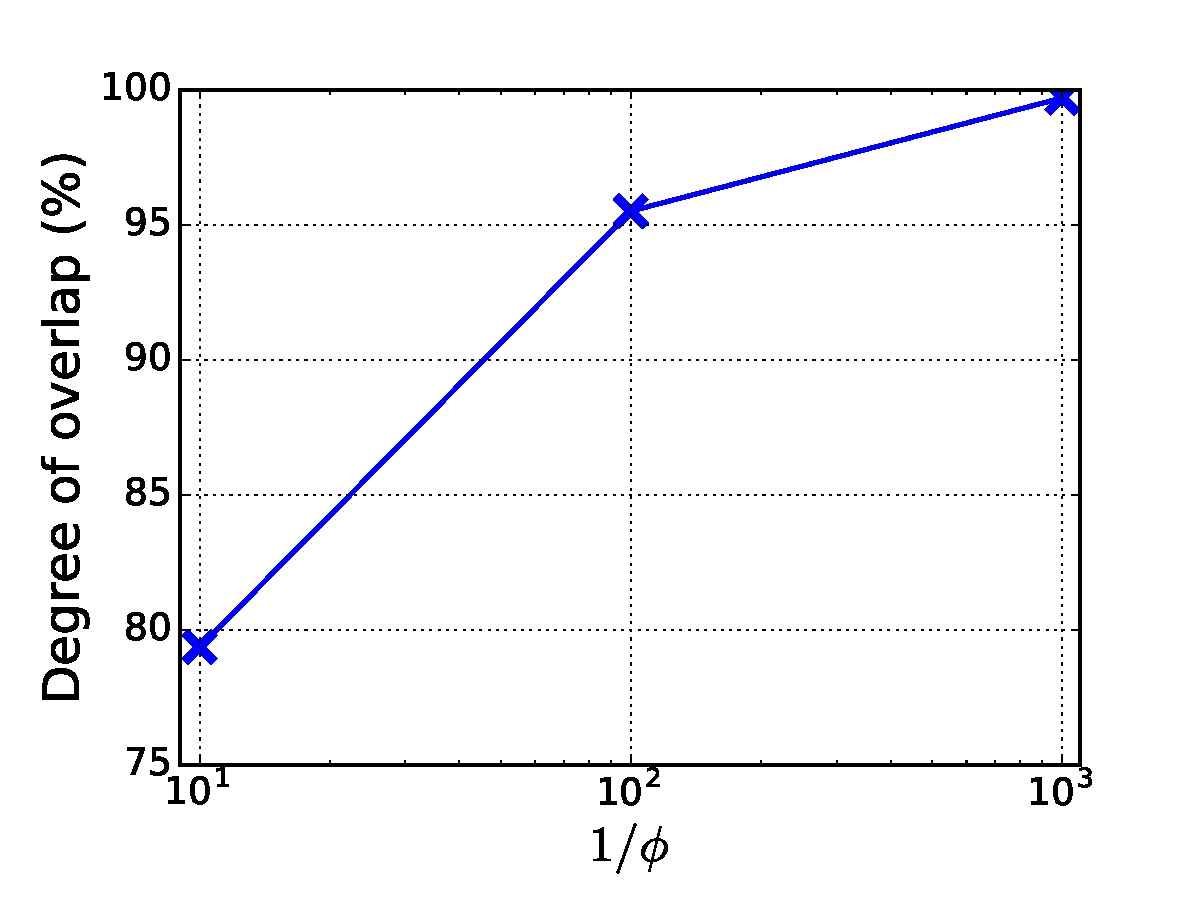
\includegraphics[width=\linewidth]{figure/overlap.pdf}
  \caption{Relation between $\phi$ and degree of overlap.}
  \label{fig:overlap}
\endminipage\hfill
\minipage{0.22\textwidth}
  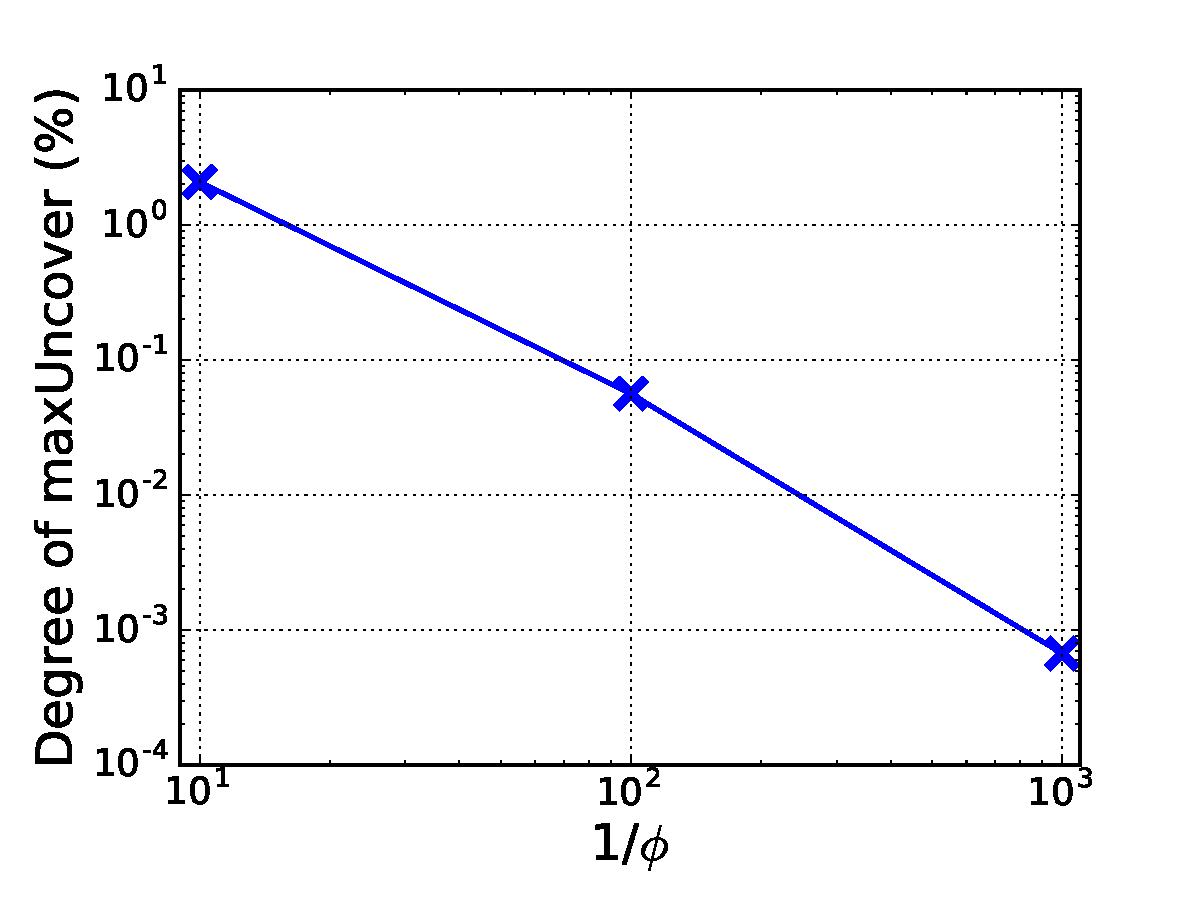
\includegraphics[width=\linewidth]{figure/maxUncover.pdf}
  \caption{Relation between $\phi$ and degree of maxUncover.}
  \label{fig:maxUncover}
\endminipage\hfill
\minipage{0.22\textwidth}%
  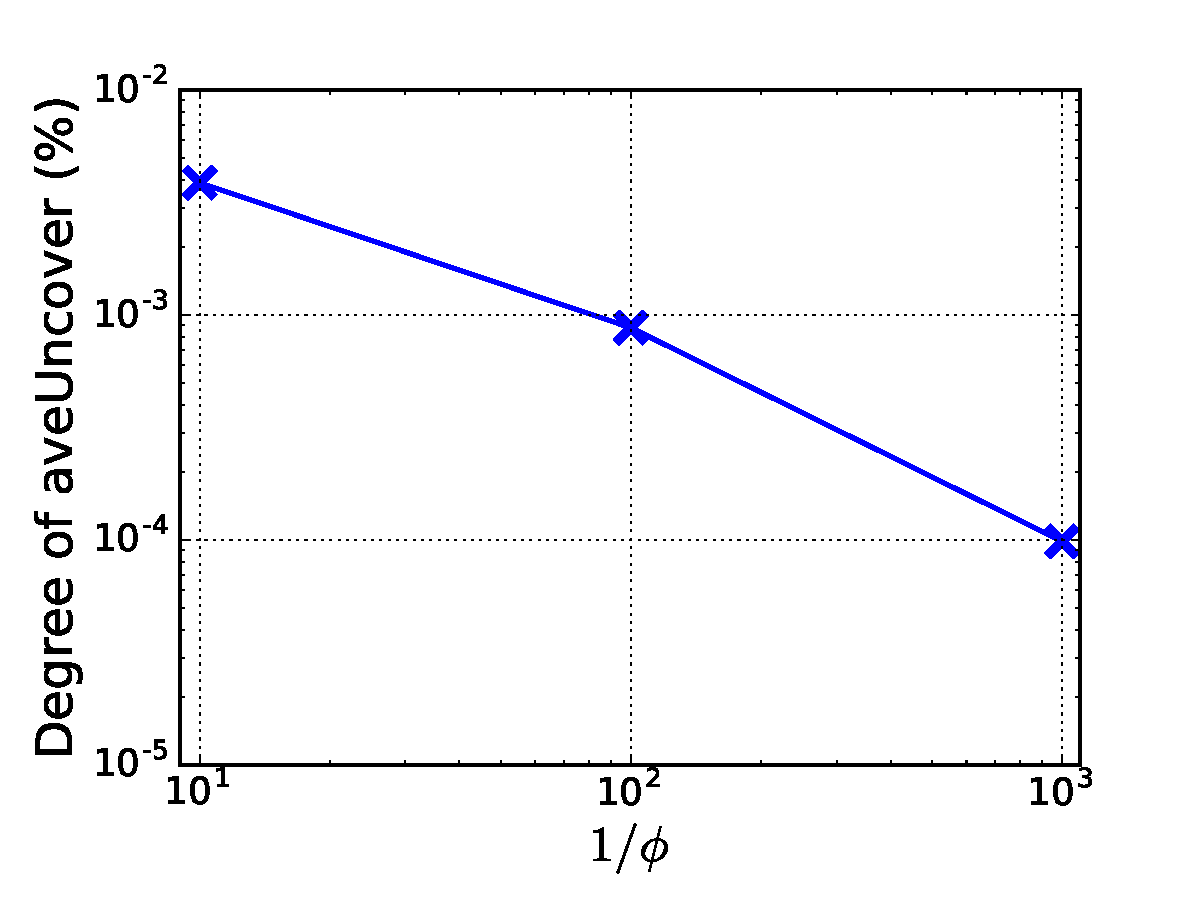
\includegraphics[width=\linewidth]{figure/aveUncover.pdf}
  \caption{Relation between $\phi$ and degree of aveUncover.}
  \label{fig:aveUncover}
\endminipage\hfill
\minipage{0.22\textwidth}%
  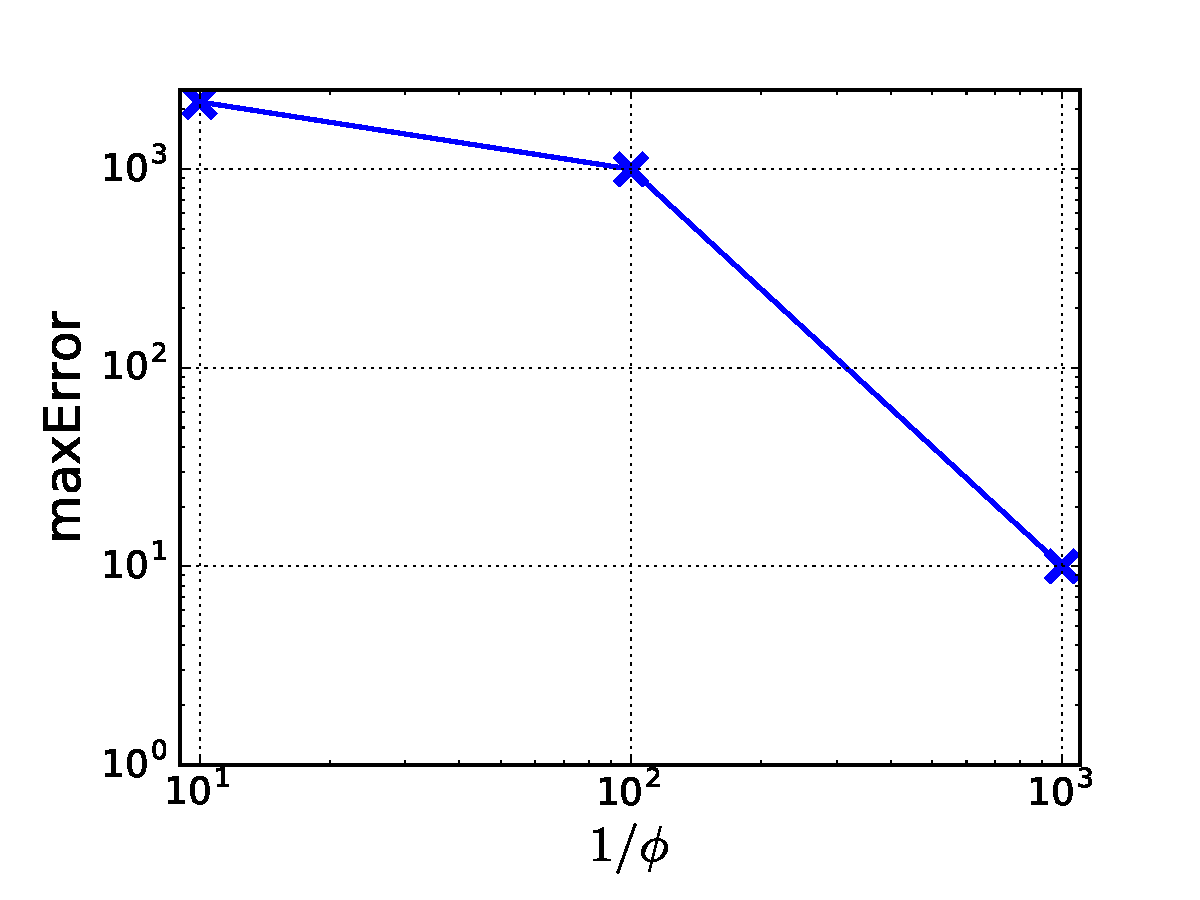
\includegraphics[width=\linewidth]{figure/maxError.pdf}
  \caption{Relation between $\phi$ and maximum error.}
  \label{fig:maxError}

\endminipage
\end{figure*}

\begin{figure}[t!]
\begin{center}
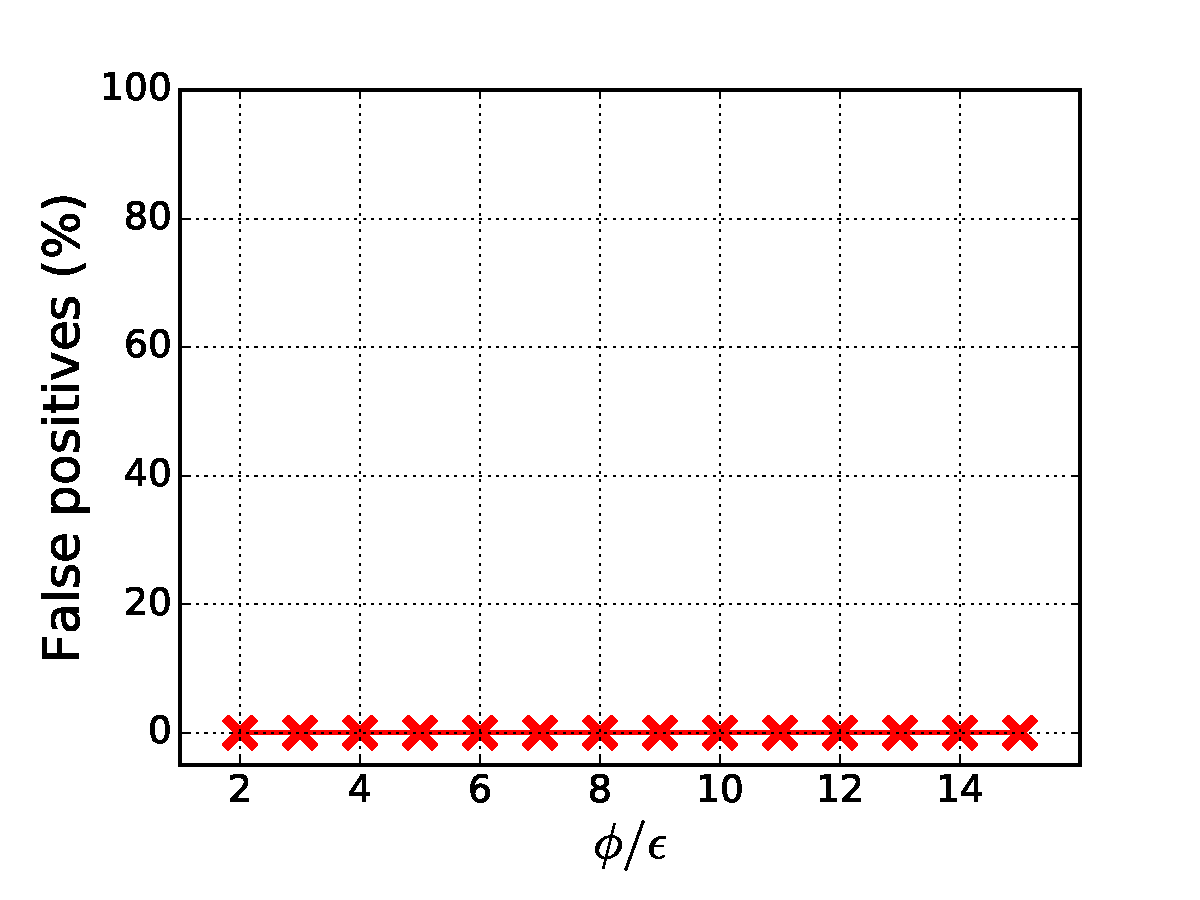
\includegraphics[width=3.0in]{figure/fp}
\caption{FP number.}
\label{fig:new}
\end{center}
\end{figure}

In this section, we view data on VirusTotal as a stream, according to each submission's timestamp, 
and apply a frequent item mining algorithm to identify hot malware family. 

Frequent item mining algorithms take two configuration parameters, $\phi$ and $\epsilon$, where $\phi > \epsilon$. 
The goal of frequent item mining algorithms are to provide nearly-real time analysis on massive data streams by using constant memory. 
Assuming the length of the input stream is N, the output of frequent item mining algorithms 
are all items which appear more than $\lfloor \phi N \rfloor$, 
and no items which appear less than  $\lfloor \epsilon N \rfloor$. 

The frequent item mining algorithm we use is space saving algorithm~\cite{space-saving}, 
which was proposed for streams in Internet advertising, and has already been applied in other areas, 
like mining hot calling contexts in profilers~\cite{hot-calling-context}.
Space saving algorithm tracks $M=1/\epsilon$ pairs of $(f, c)$. 
$f$ is short for malware family, and $c$ is short for counter.  
Pair content represents $(\phi, \epsilon)\mbox{-}HMF$ (Hot Malware Family). 
The M pairs are initialized with the first M encountered malware families and their frequency. 
When a new malware submission comes, 
if the malware family is already under monitored, 
the related counter will be increased by 1. 
And if the malware family is not monitored, 
we will replace the malware family of the pair with lowest counter value with the new malware family, 
and increase its counter value by 1. 
When querying HMF, 
all malware families whose counter values are larger than $\lfloor \phi N \rfloor$ will be returned. 


Following previous works in frequent item mining~\cite{hot-calling-context}, 
we will measure the following metrics by using malware submission date we collect:

Degree of \textit{overlap} is used to measure the percentage of malwares covered in $(\phi, \epsilon)\mbox{-}HMF$,
and it is defined as follows:

$$overlap((\phi, \epsilon)\mbox{-}HMF) = \dfrac{1}{N}\sum_{f \in (\phi, \epsilon)\mbox{-}HMF}w(f)$$

In the above equation, $N$ represents the total number of malware submissions, and 
$w(f)$ represents the real frequency of malware family $f$.  

\textit{maxUncover} (maximum frequency of uncovered malware families) and 
is used 
to measure largest frequency of malware familiy not covered in $(\phi, \epsilon)\mbox{-}HMF$. 
They are defined as follows:
$$maxUncover((\phi, \epsilon)\mbox{-}HMF) = \max_{f \notin (\phi, \epsilon)\mbox{-}HMF}w(f)$$

\textit{aveUncover} (average frequency of uncovered malware families) is defined similarly. 

\textit{False positives} are defined as malware families returned during querying HMF, but whoese
real frequencies are less than $\lfloor \phi N \rfloor$. 

\textit{maxError} is used to measure relative error of counter values, compared with real frequencies.
It is defined as follows:

$$maxError((\phi, \epsilon)\mbox{-}HMF) = \max_{f \in (\phi, \epsilon)\mbox{-}HMF} \dfrac{\left|c(f) - w(f)\right|}{w(f)}$$






\section{Research Opportunities}
\label{sec:oppo}
Beyond the research described above, we illustrate a number of research opportunities as follows: 

{\bf Utilizing other metadata fields.} 
We currently only leverage timestamp and Microsoft detection reports. 
There are many other metadata fields. 
Conducting data mining on these fields could enable 
Many other ``big security'' applications. 
For example, there are existing techniques leverage submission\_id information to identify malware writers~\cite{neeles}. 
For example, future research could leverage ssdeep information to cluster malwares, 
and conduct malware prediction and hot malware mining in a finer granularity. 

{\bf Utilizing other antivirus vendors’ reports.}
We currently only leverage reports from Microsoft, but these reports may not be always accurate.
There are more than 40 antivirus vendors' reports also provided on VirusTotal.
Some vendors’ reports may be better than others, or better than others under some special conditions. 
We leave systematically evaluating all those reports and better combining reports from different vendors in the future. 

{\bf Improving antivirus products.} 
There are also opportunities to improve existing antivirus products. 
For example, many endpoint antivirus softwares, like ClamAV, are built based on a database of malwares' signatures. 
When these antivirus softwares scan suspicious files, all signatures in the database will be checked. 
If we can precisely predict which malware would appear in the near future, 
we could reduce the size of signatures sent to clients' side and also reduce time to check the signature database. 

{\bf Studying other types of malicious files. }
Besides PE files, there are other types of malicious files on VirusTotal, like malicious apps, 
malicious URL, and malicious binary files on other systems. 
What are the characteristics of these files and whether they follow the same patterns as PE files remain an open issue.  
\section{Related works}

Many research efforts~\cite{bigcode, big-lessons,big-translation,code-completion,big-predicting} 
have been made to explore how to leverage ``big code'' repositories, 
such as GitHub, BitBucket, and CodePlex, and these works inspire us to explore how to leverage data on VirusTotal. 
SLANG~\cite{code-completion} can fill uncompleted programs with call innovations 
by using statistical models trained from extracted sequences of API calls from large code bases.  
JSNICE~\cite{big-predicting} can predict identifier types and obfuscated identifier names for Javascript programs. 
JSNICE translates programs into dependence graphs and learns a CRF model by using a large training set. 
All predictions are made by optimizing a score function based on the learned CRF model. 
\citet{big-translation} apply phrase-based statistical translation approaches to translate C\# programs to Java.
To sum up, all these techniques are built based on source code repositories, 
and their goals are to improve the development stage. 
However, VirusTotal is a repository containing binary malwares
and the goal for conducting data mining on VirusTotal data is to improve antivirus techniques. 

There are existing works~\cite{hacker-vt,neeles} regarding the conducting of data mining on VirusTotal data to identify malware development cases, 
where malware writers use VirusTotal as a testing platform and 
try to develop malwares that cannot be detected by antivirus engines. 
These techniques utilize submission\_id information, which is different from the information we use. 
We believe other information on VirusTotal could also be leveraged in the future. 


\section{Conclusion}
Data on VirusTotal has largely been ignored by research community. 
In this paper, we conduct an empirical study on PE malwares on VirusTotal. 
Our study is mainly performed to understand the temporal characteristics and
the family distribution characteristics of malwares. We also build two techniques, 
cache-based malware prediction and hot malware family mining, to validate our observations. 
We expect our work to deepen our understanding of and bring more attention to the data on VirusTotal. 
%\input{related}
%\input{conclusion}

%%\balance
%\begin{spacing}{0.65}

\balance
{
\bibliographystyle{abbrvnat}
\bibliography{security} 
}
%\end{spacing}
\end{document}

% Local variables:
% TeX-PDF-mode: t
% TeX-master: t
% End:

% LocalWords:  Crug cci
